\documentclass{beamer}
\usepackage{amsmath}
\usepackage{listings}
\usepackage{listings}
\usepackage{floatflt}
\usepackage{qtree}
\lstset{language=Haskell,basicstyle=\ttfamily}
%\usepackage{beamerthemesplit}
\usetheme{Szeged}
 
\title{Self-adjusting heaps}
\subtitle{A comparison}
\author{Johan Brinch \and Asser Femø}
\date{\today}
\newcommand{\bind}{\texttt{>>=}}
\newcommand{\ret}{\texttt{return}}
\newcommand{\bs}{\texttt{\char`\\}}
\newcommand{\fs}{\char`/}
\newcommand{\at}{\texttt{a}}
\newcommand{\kt}{\texttt{k}}
\newcommand{\mt}{\texttt{k}}
\begin{document}
\lstset{basicstyle=\footnotesize\ttfamily}
%\section*{Introduction}
\begin{frame}
  \titlepage
\end{frame}
 
\section{The Pairing Heap}
\subsection{Overview}
\begin{frame}[fragile]
\frametitle{Pairing Heap}

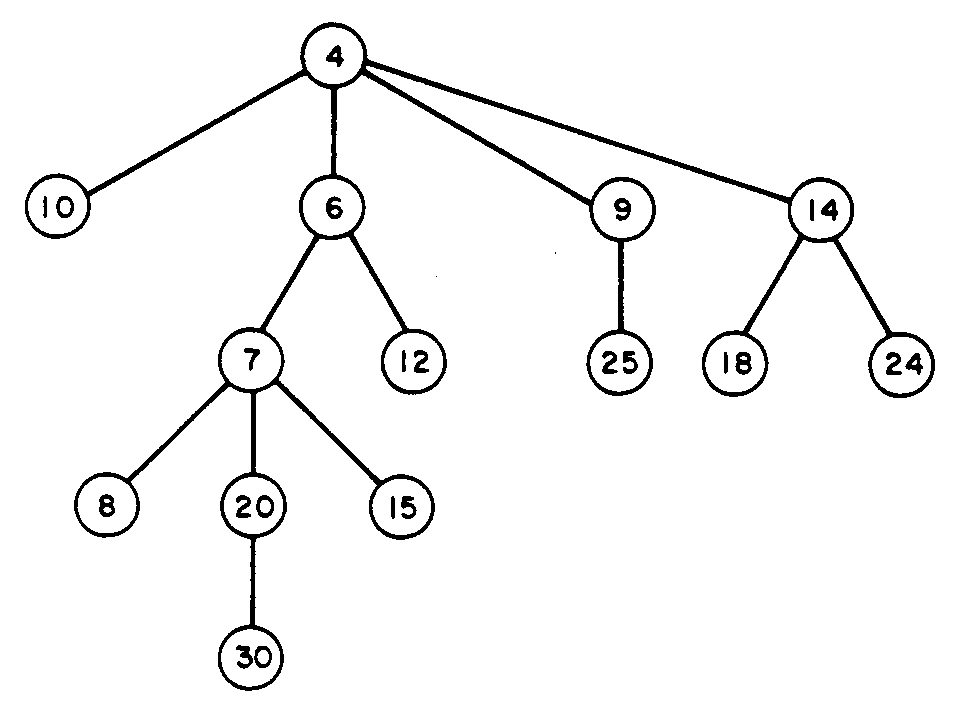
\includegraphics[width=7cm]{../pairing-heap-slides/fig1.png}

\end{frame}

\begin{frame}
\frametitle{Operations}

\begin{description}
\item[link] make the root of smaller key the parent of the root of larger key
\item[insert] make $x$ a single-node tree and link with $H$
\item[delete-min] delete root of $H$, link its children
\item[find-min] return root of $H$
\item[decrease-key] decrease key of $x$, cut $x$ from $H$ and link them
back together
\item[delete] cut $x$ from $H$, do delete-min on $x$ and link its children to $H$
\end{description}

\end{frame}

\begin{frame}
\frametitle{Child-sibling representation}
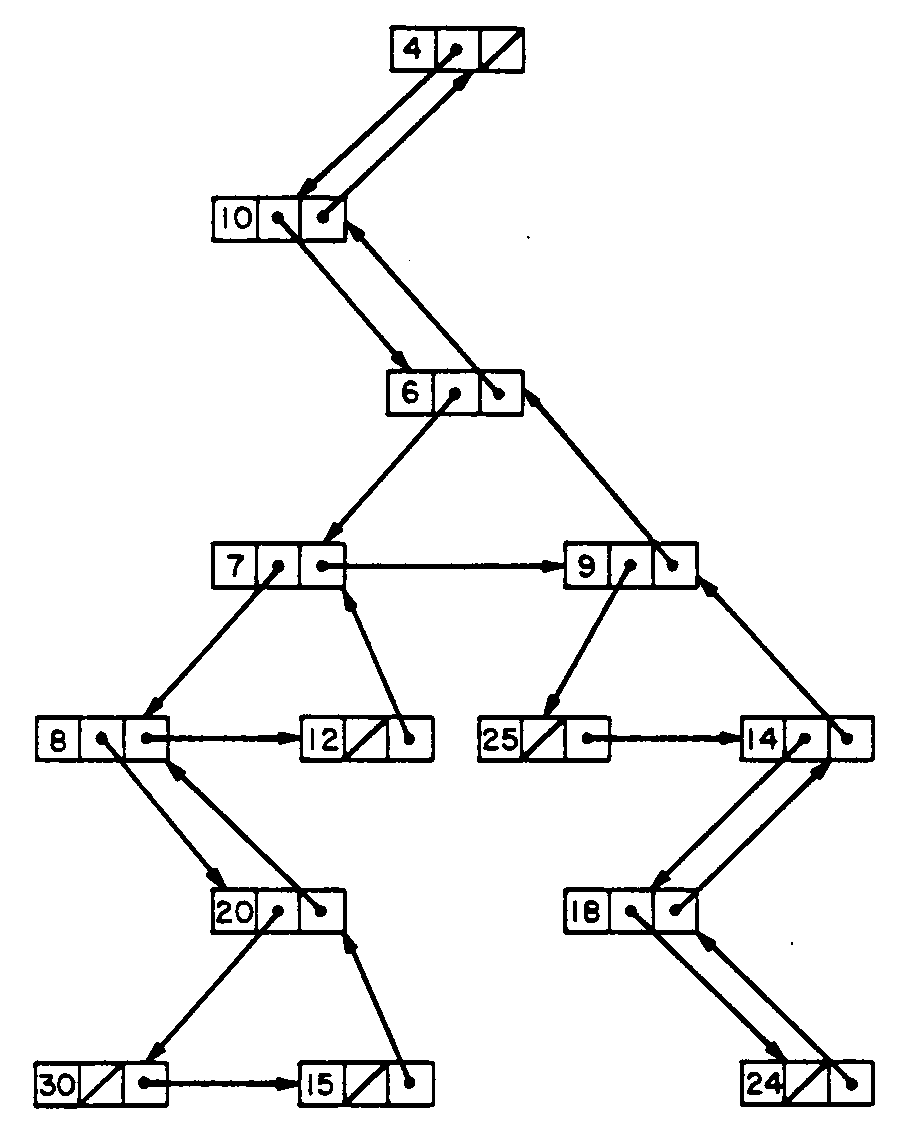
\includegraphics[width=5cm]{../pairing-heap-slides/fig3.png}

\end{frame}

\begin{frame}
\frametitle{Running times}

\textbf{find-min}, \textbf{insert}, \textbf{meld} and \textbf{decrease-key} 
run in $O(1)$ worst-case time.

\textbf{delete-min} and \textbf{delete} run in worst case $\Theta(n)$ time but
can be improved to $O(\log n)$ amortized time by two-pass or multipass linking.

\end{frame}

\begin{frame}
\frametitle{Variants}

\textbf{Stasko-Vitter Lazy Insertion}

Insert into auxiliary buffer. After \textbf{delete-min} multipass link the
buffer contents and link with main tree.

Improves \textbf{insert} to amortized $O(1)$ time.

\end{frame}

\begin{frame}
\frametitle{Variants}

\textbf{Elmasry Costless Meld}\\

\textbf{decrease-key} adds node to auxiliary decrease buffer. Following
\textbf{meld} and \textbf{delete-min} clean up the decrease buffer cutting
decreased nodes from the main tree, combining and linking them back into the
main tree.

Improves \textbf{decrease-key} $O(\log \log n)$ amortized time and \textbf{meld}
to zero amortized time.

\end{frame}

\begin{frame}
\frametitle{Amortized running times}

\begin{tabular}{|c|c|c|c|c|}
\hline
& \textbf{insert} & \textbf{delete-min} & \textbf{decrease-key} & \textbf{meld} \\
\hline
Original & $O(\log n)$ & $O(\log n)$ & $O(\log n)$ & $O(\log n)$ \\
\hline
Lazy insertion & $O(1)$ & $O(\log n)$ & $O(\log n)$ & $O(\log n)$ \\
\hline
Costless meld & $O(1)$ & $O(\log n)$ & $O(\log \log n)$ & zero \\
\hline
\end{tabular}

\end{frame}
 
\end{document}
 
